\chapter{Anubis Cloud IDEs}\label{ch:cloud_ides}

\begin{figure}[ht]
    \centering
    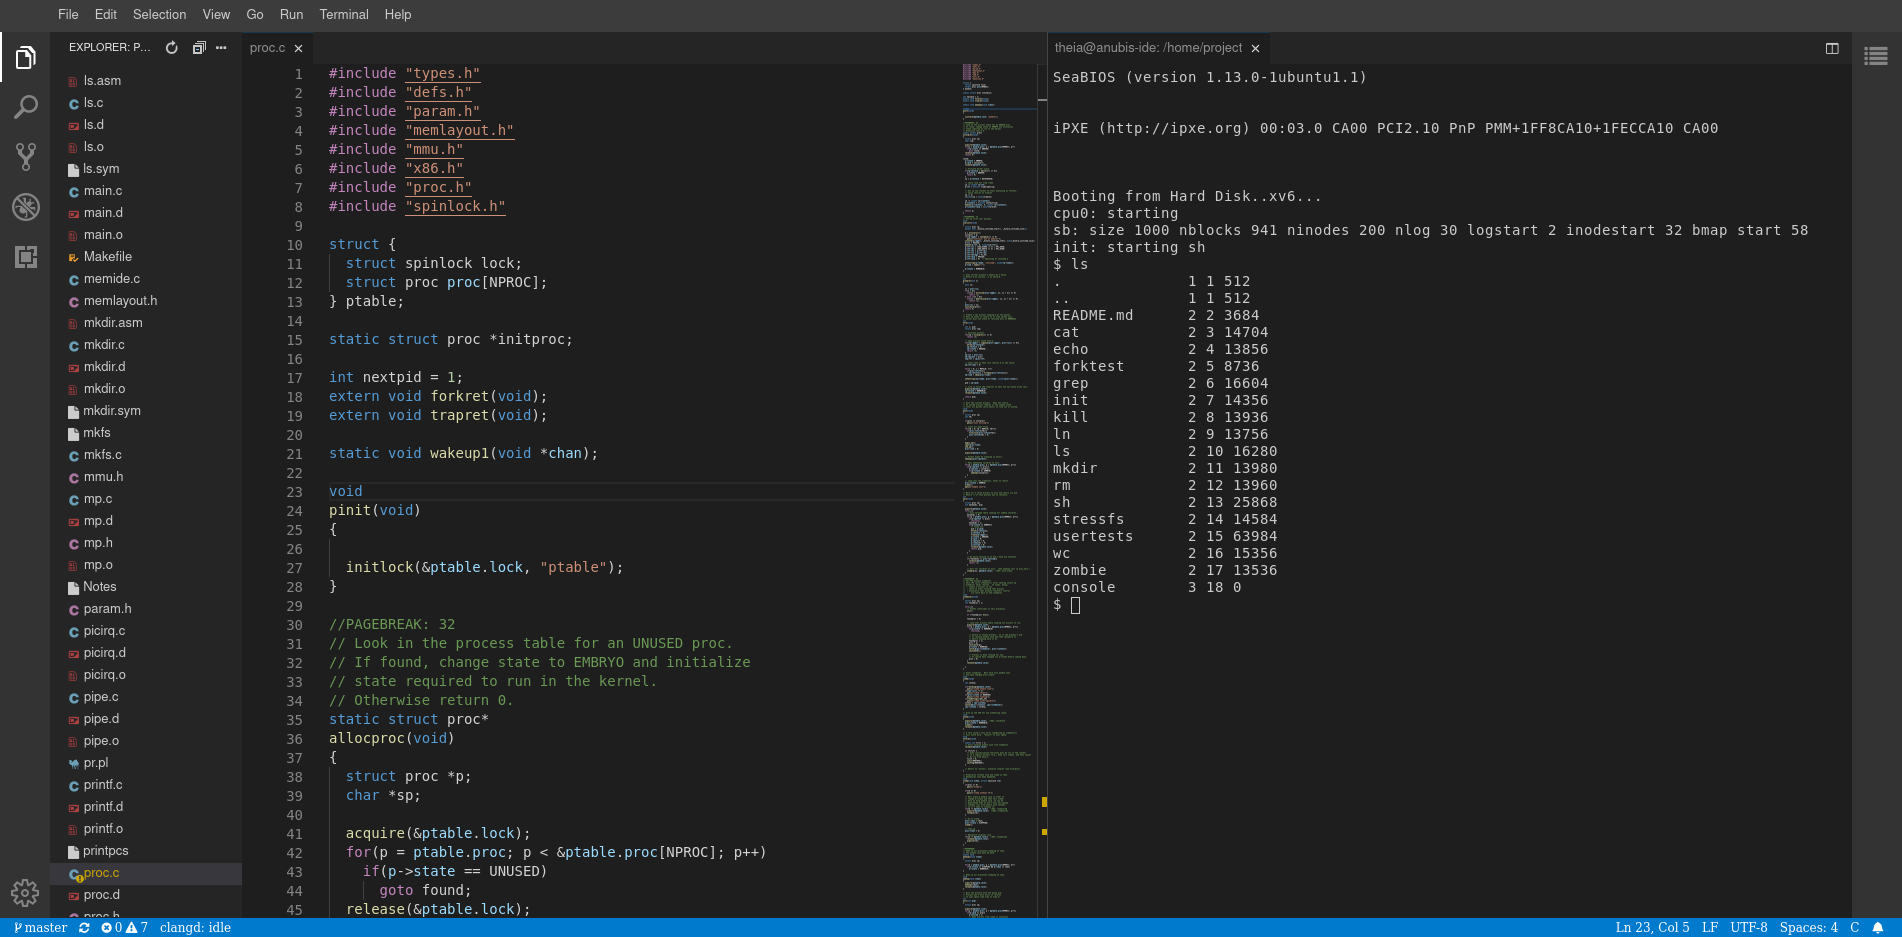
\includegraphics[width=0.9\textwidth]{figures/theia2}
    \caption{Anubis Cloud IDE\label{fig:theia2}}
\end{figure}

\section{Cloud IDE Overview}\label{sec:cloud-ide-overview}

One of the more exciting new features of Anubis is that of the Cloud IDEs.
Anubis Cloud IDEs are \href{https://theia-ide.org/}{Theia} IDE servers that run in containers.
Since the containers are themselves linux environments, we can allow students
to run commands in that environment with the built in terminal in Theia.

\section{Packaging of Course Software}\label{sec:packaing-of-course-software}

Taking these IDE container servers to the next level, we can add whatever 
other software is necessary for the course.
Packaging the tools that students need into a custom Theia server container
built specifically for the needs of the course are then available with 
one click to students.
Nothing to install, nothing to setup.
All students need is a modern web browser and an internet connection.

For many years, the CS-UY 3224 (Intro. to Operating Systems) course
jumped around from one VM solution to another.
Each one posed challenges with setting up for some subset of students.
By using the Anubis IDEs, this issue is completely removed.
The tools necessary for the homeworks are packaged into the of build 
of Theia that is used for the course.
The course VMs are then no longer necessary.
Students have access to all the tools they need through the Cloud IDE
with one click.

\section{IDE Guarantees}\label{sec:ide-garantees}

Leveraging some magic that Kubernetes and containers give us,
we can provide a fully insulated linux environment for hundreds of
students concurrently.

Any solution in the cloud that we provide for student need certain assurances.
The majority of students will rely on the Cloud IDEs to do their homework.
The system cannot fail right before a deadline when the load on Anubis is greatest.
Cloud IDEs need to be scalable.
This requires the system to distribute Cloud IDE instances across multiple nodes. 
Networking traffic to Cloud IDEs need to also be automatically detected and balanced.

\subsection{Scaling IDEs}\label{subsec:scaling-ides}

Kubernetes tracks what resources are reserved for specific containers.
When it runs out of a resource like memory of cpu, it will automatically
add more nodes to the cluster and spread the load.
There resource reservations are added to each student Cloud IDE.
If there are more students asking for Cloud IDEs resources than exist
in the cluster, it will automatically scale to handle the load.

\subsection{Balancing Network Traffic}\label{subsec:balancing-network-traffic}

There is a service in Anubis whose only purpose is to route
student requests to IDE instances. 
This service is called the \textit{theia-proxy}. 
See~\fref{fig:anubis-ide} to see where the \textit{theia-proxy}
fits into the deployment.

\begin{figure}
    \centering
    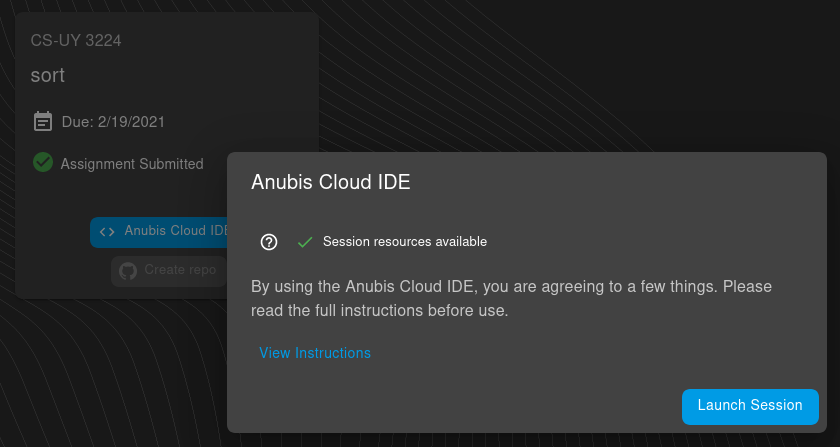
\includegraphics[width=0.5\textwidth]{figures/theia1.png}
    \caption{Launch Anubis Cloud IDE\label{fig:theia1}}
\end{figure}

When a student clicks the button to create a Cloud IDE, 
an IDE pod is created for that student~\fref{fig:theia1}.
At the time that the pod is created, the in cluster ip address
of that pod is recorded in the database (called a \textit{ClusterIP}).

Once the Cloud IDE has been initialized, then a \textit{goto ide} button
will become available.
When clicked, the student will be redirected to \textit{ide.anubis.osiris.services}.
That domain points to the \textit{theia-proxy} service.
The proxy then parses the cookie set for the user, and pulls the 
cloud ide pod ip address from the database.
The proxy then forwards the request to the proper Cloud IDE container.

The \textit{theia-proxy} service is setup with a 
\href{https://kubernetes.io/docs/tasks/run-application/horizontal-pod-autoscale/}{Horizontal Pod Autoscaler} or HPA.
These are special kubernetes resources that will automatically add or subtract containers
from a deployment based on the resources in use.
The HPA for the \textit{theia-proxy} is configured to detect when 
there is prolonged cpu load and automatically add new proxy containers.
The load balancer will then automatically distribute incomming connections
between \textit{theia-proxy} containers.


\section{IDE Pod Design}\label{sec:ide-pod-design}

\begin{figure}[ht]
    \centering
    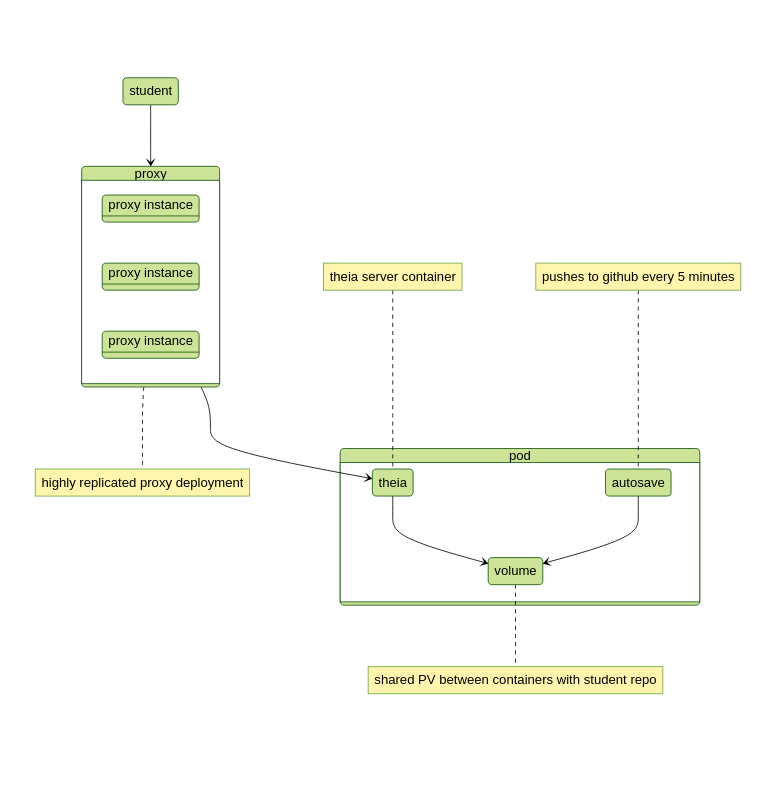
\includegraphics[width=0.5\textwidth]{figures/theia-pod.mmd}
    \caption{Anubis Cloud IDE design\label{fig:anubis-ide}}
\end{figure}

The Cloud IDE pod design requires some finesse. 
There are a couple of things about theia that make it so that
we need to do some rather fancy things in Kubernetes to make 
the setup work.

The main thing that we need to handle is the fact that theia requires a websocket connection between the browser and
theia server instance. When the pods are allocated Anubis records the ClusterIP in the database. Then when we need to
initialize a client connection Anubis uses this saved ClusterIP to forward requests (both http and websockets) to the
correct pod.

These IDE servers are temporary. When the student finishes working (or after a timeout) we reclaim the resources by
deleting the pod and shared volume. Because of this, we needed some form of autosave. Saving is pushing to github.
The issue we need to contend with is automatically committing and pushing to github without exposing a sensitive
password or api token to the users. We handle this by having a second container whose only role is committing and
pushing to github. The credentials live in that container, completely separate and inaccessible to the user who
may be working in the other theia server container. These two containers are connected by a shared volume mounted
at `/home/project` in both containers. This volume is relatively small (~50MiB).

With this setup, we have autosave running in the background while being completely hidden from the user. When
explaining autosave to students we usually just say "it is witchcraft, just trust that it works".


With these lightweight containerized theia servers, we are able to support significantly more concurrent users than
if we had elected to implement a cloud VM solution. Because Anubis Cloud IDEs do not need to virtualize hardware,
the resources on the system for each user is significantly less. Given the resources that we have on Digital Ocean,
we would be able to have maybe 20-30 concurrent users using cloud virtual machines. With our containerized theia,
we can handle all ~130 students in CS-UY 3224 at the same time with room to breath.
